%!TEX program = xelatex
\documentclass{beamer}

\RequirePackage{listings}

% Don't delete:
\newif\ifsplit
% It is necessary for switching from one outer theme to the other. By default, a miniframes outer theme is used for the header.
% Uncomment the following line to switch to a split outer theme:
\splittrue
% I suggest using the split outer theme if subsections are meaningful, miniframes otherwise.

\lstset{
  basicstyle=\tiny\ttfamily,
  escapechar=*,
  framesep=4pt,
  breakatwhitespace=true,
  keywordstyle=\color{blue}\tiny\bfseries,
  breakindent=2ex,
  morekeywords={}
}

\resetcounteronoverlays{lstlisting}

\usetheme{Theme}

\title{compile-beamer}
\subtitle{with SciLifeLab template}
\author{MaxUlysse}
\institute{Barntumörbanken / SciLifeLab}
\date{2016/12/02}

\begin{document}

\begin{frame}[noframenumbering, plain]
	\titlepage
\end{frame}

\begin{frame}[fragile]
\frametitle{compile-beamer}
Just a simple beamer compiler with Nextflow
\begin{lstlisting}[title=Usage]
nextflow run main.nf --tex <file.tex> --theme <BTB || KI || SLL> \
[--pictures <pictures directory>]
\end{lstlisting}
\begin{lstlisting}[title=This file was made using]
nextflow run main.nf --tex sample.tex --theme SLL
\end{lstlisting}
\end{frame}

\begin{frame}[fragile]
\frametitle{How to insert picture}
\begin{lstlisting}[title=Code]
\begin{center}
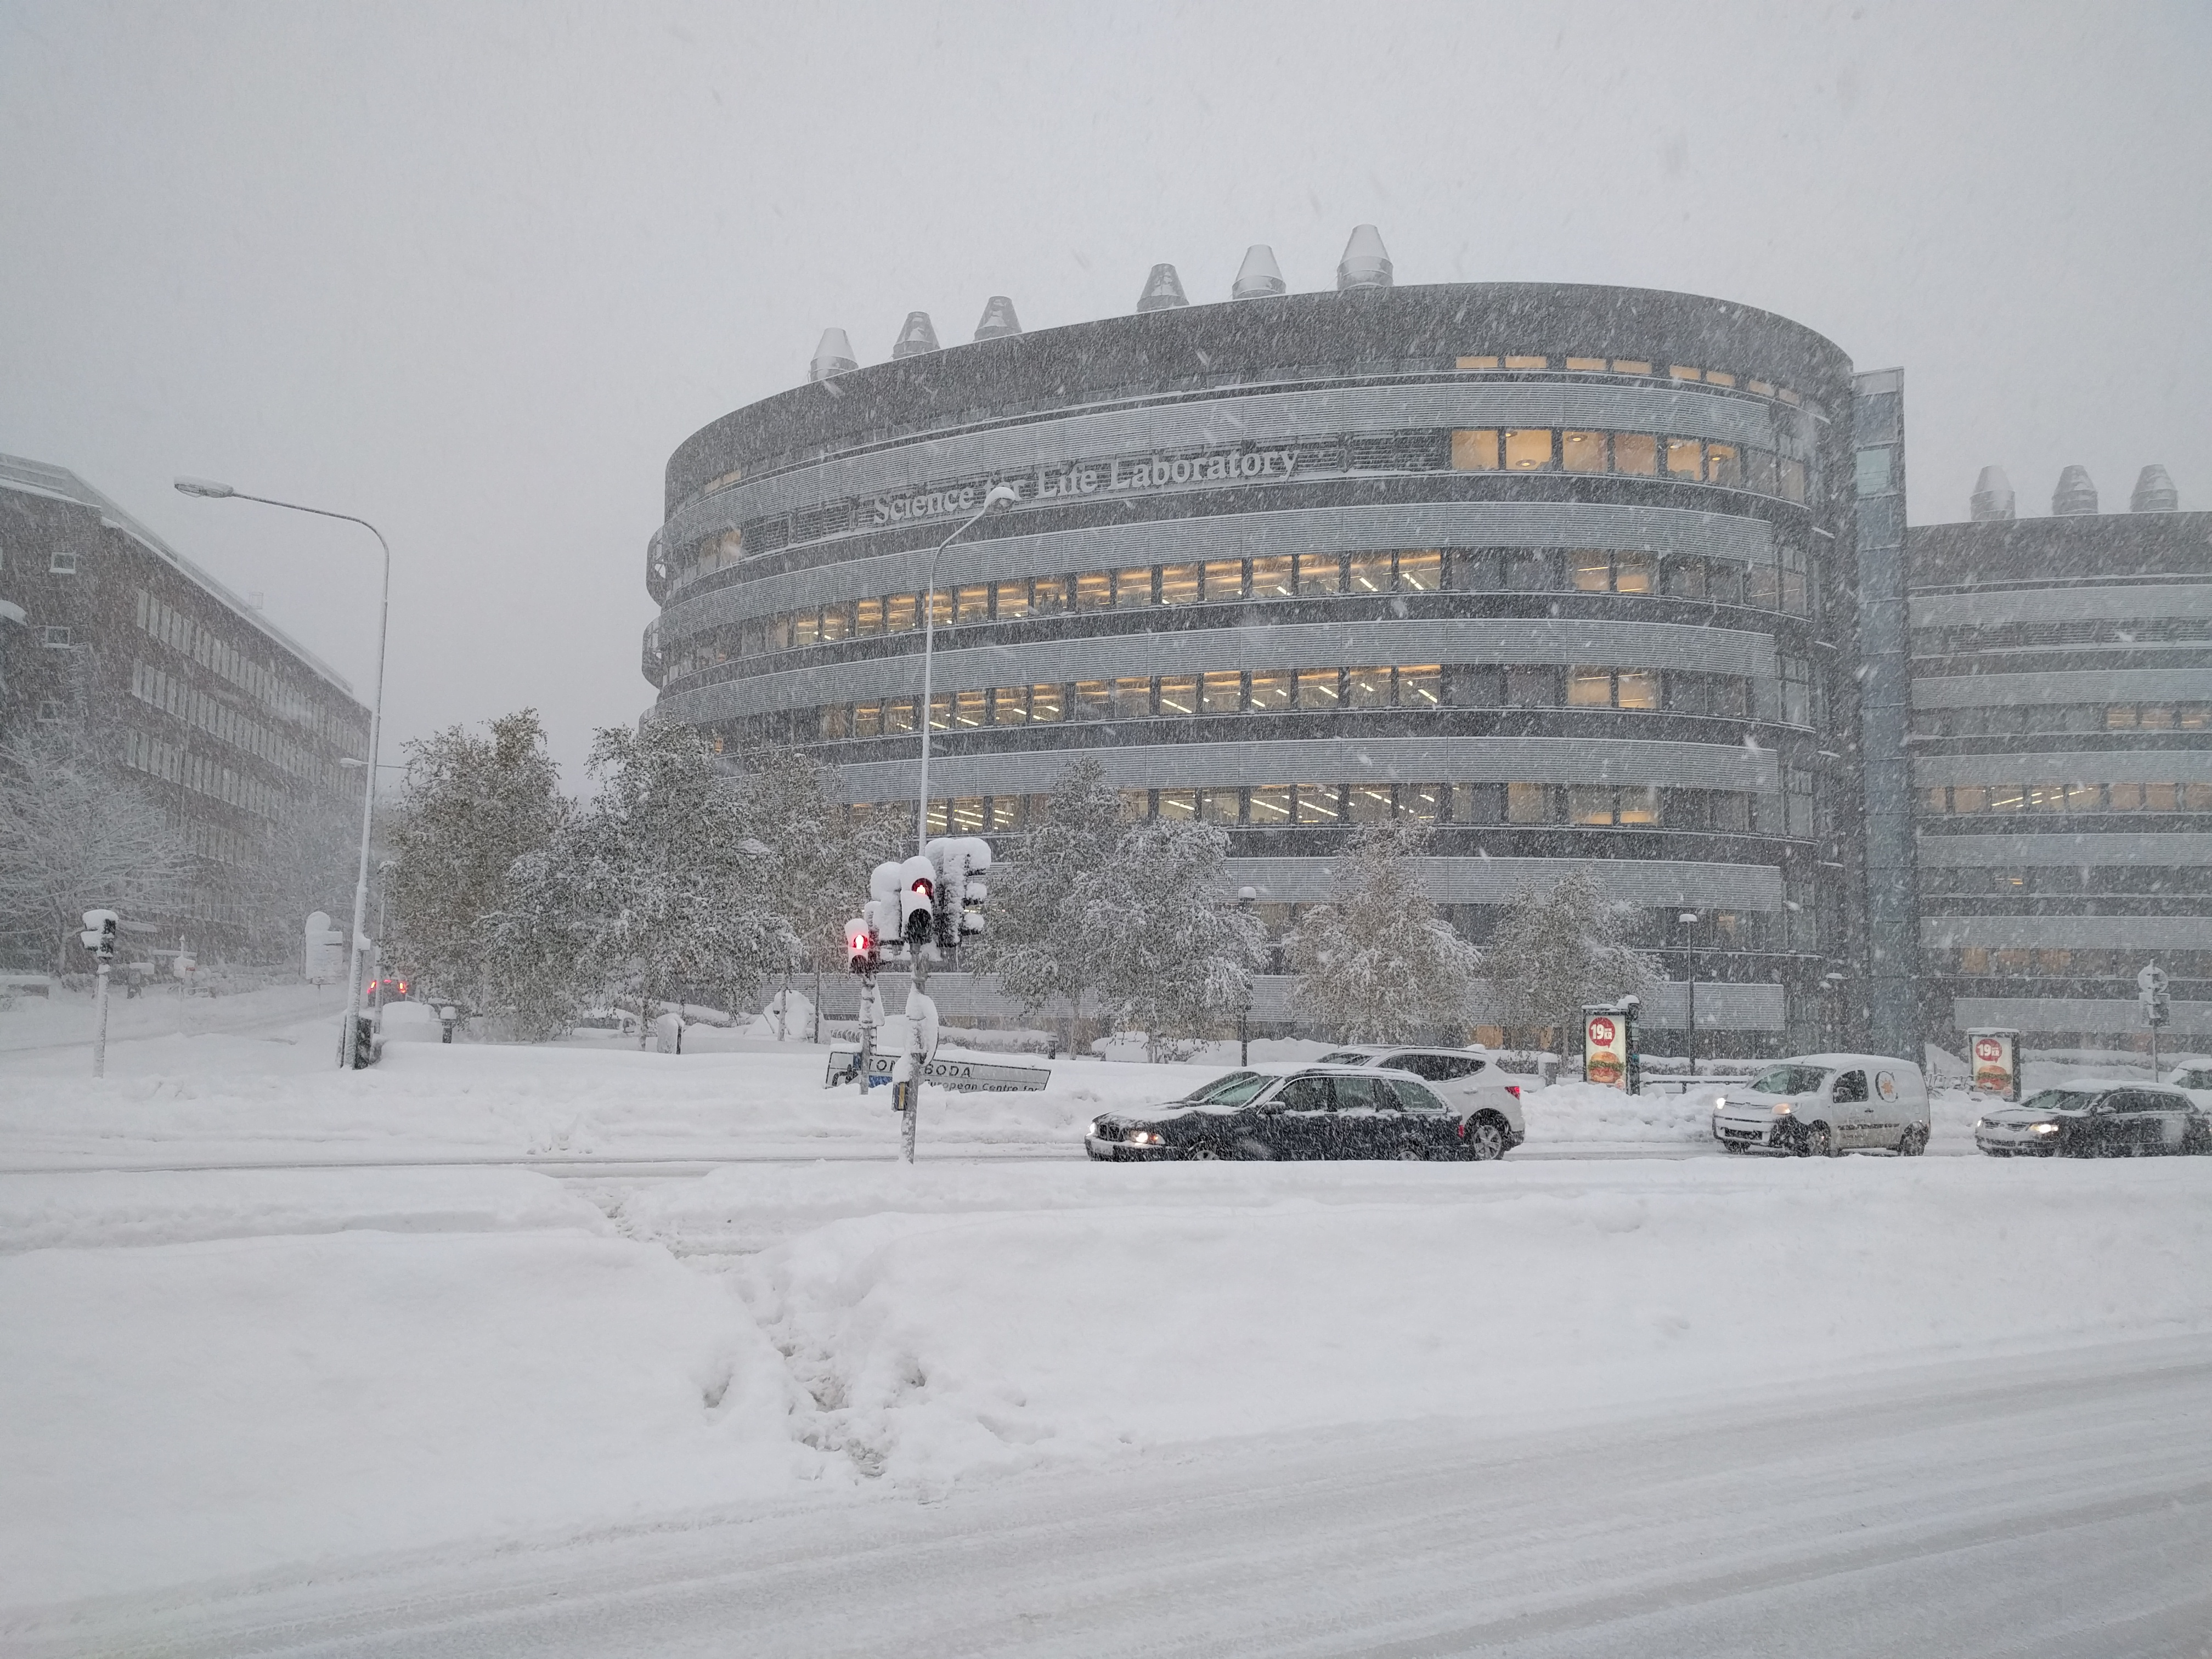
\includegraphics[width=.8\linewidth]{pictures/Snowpocalypse-SciLifeLab.jpg}
\end{center}
\end{lstlisting}
\end{frame}

\begin{frame}
	\frametitle{How to insert picture}
	\begin{center}
		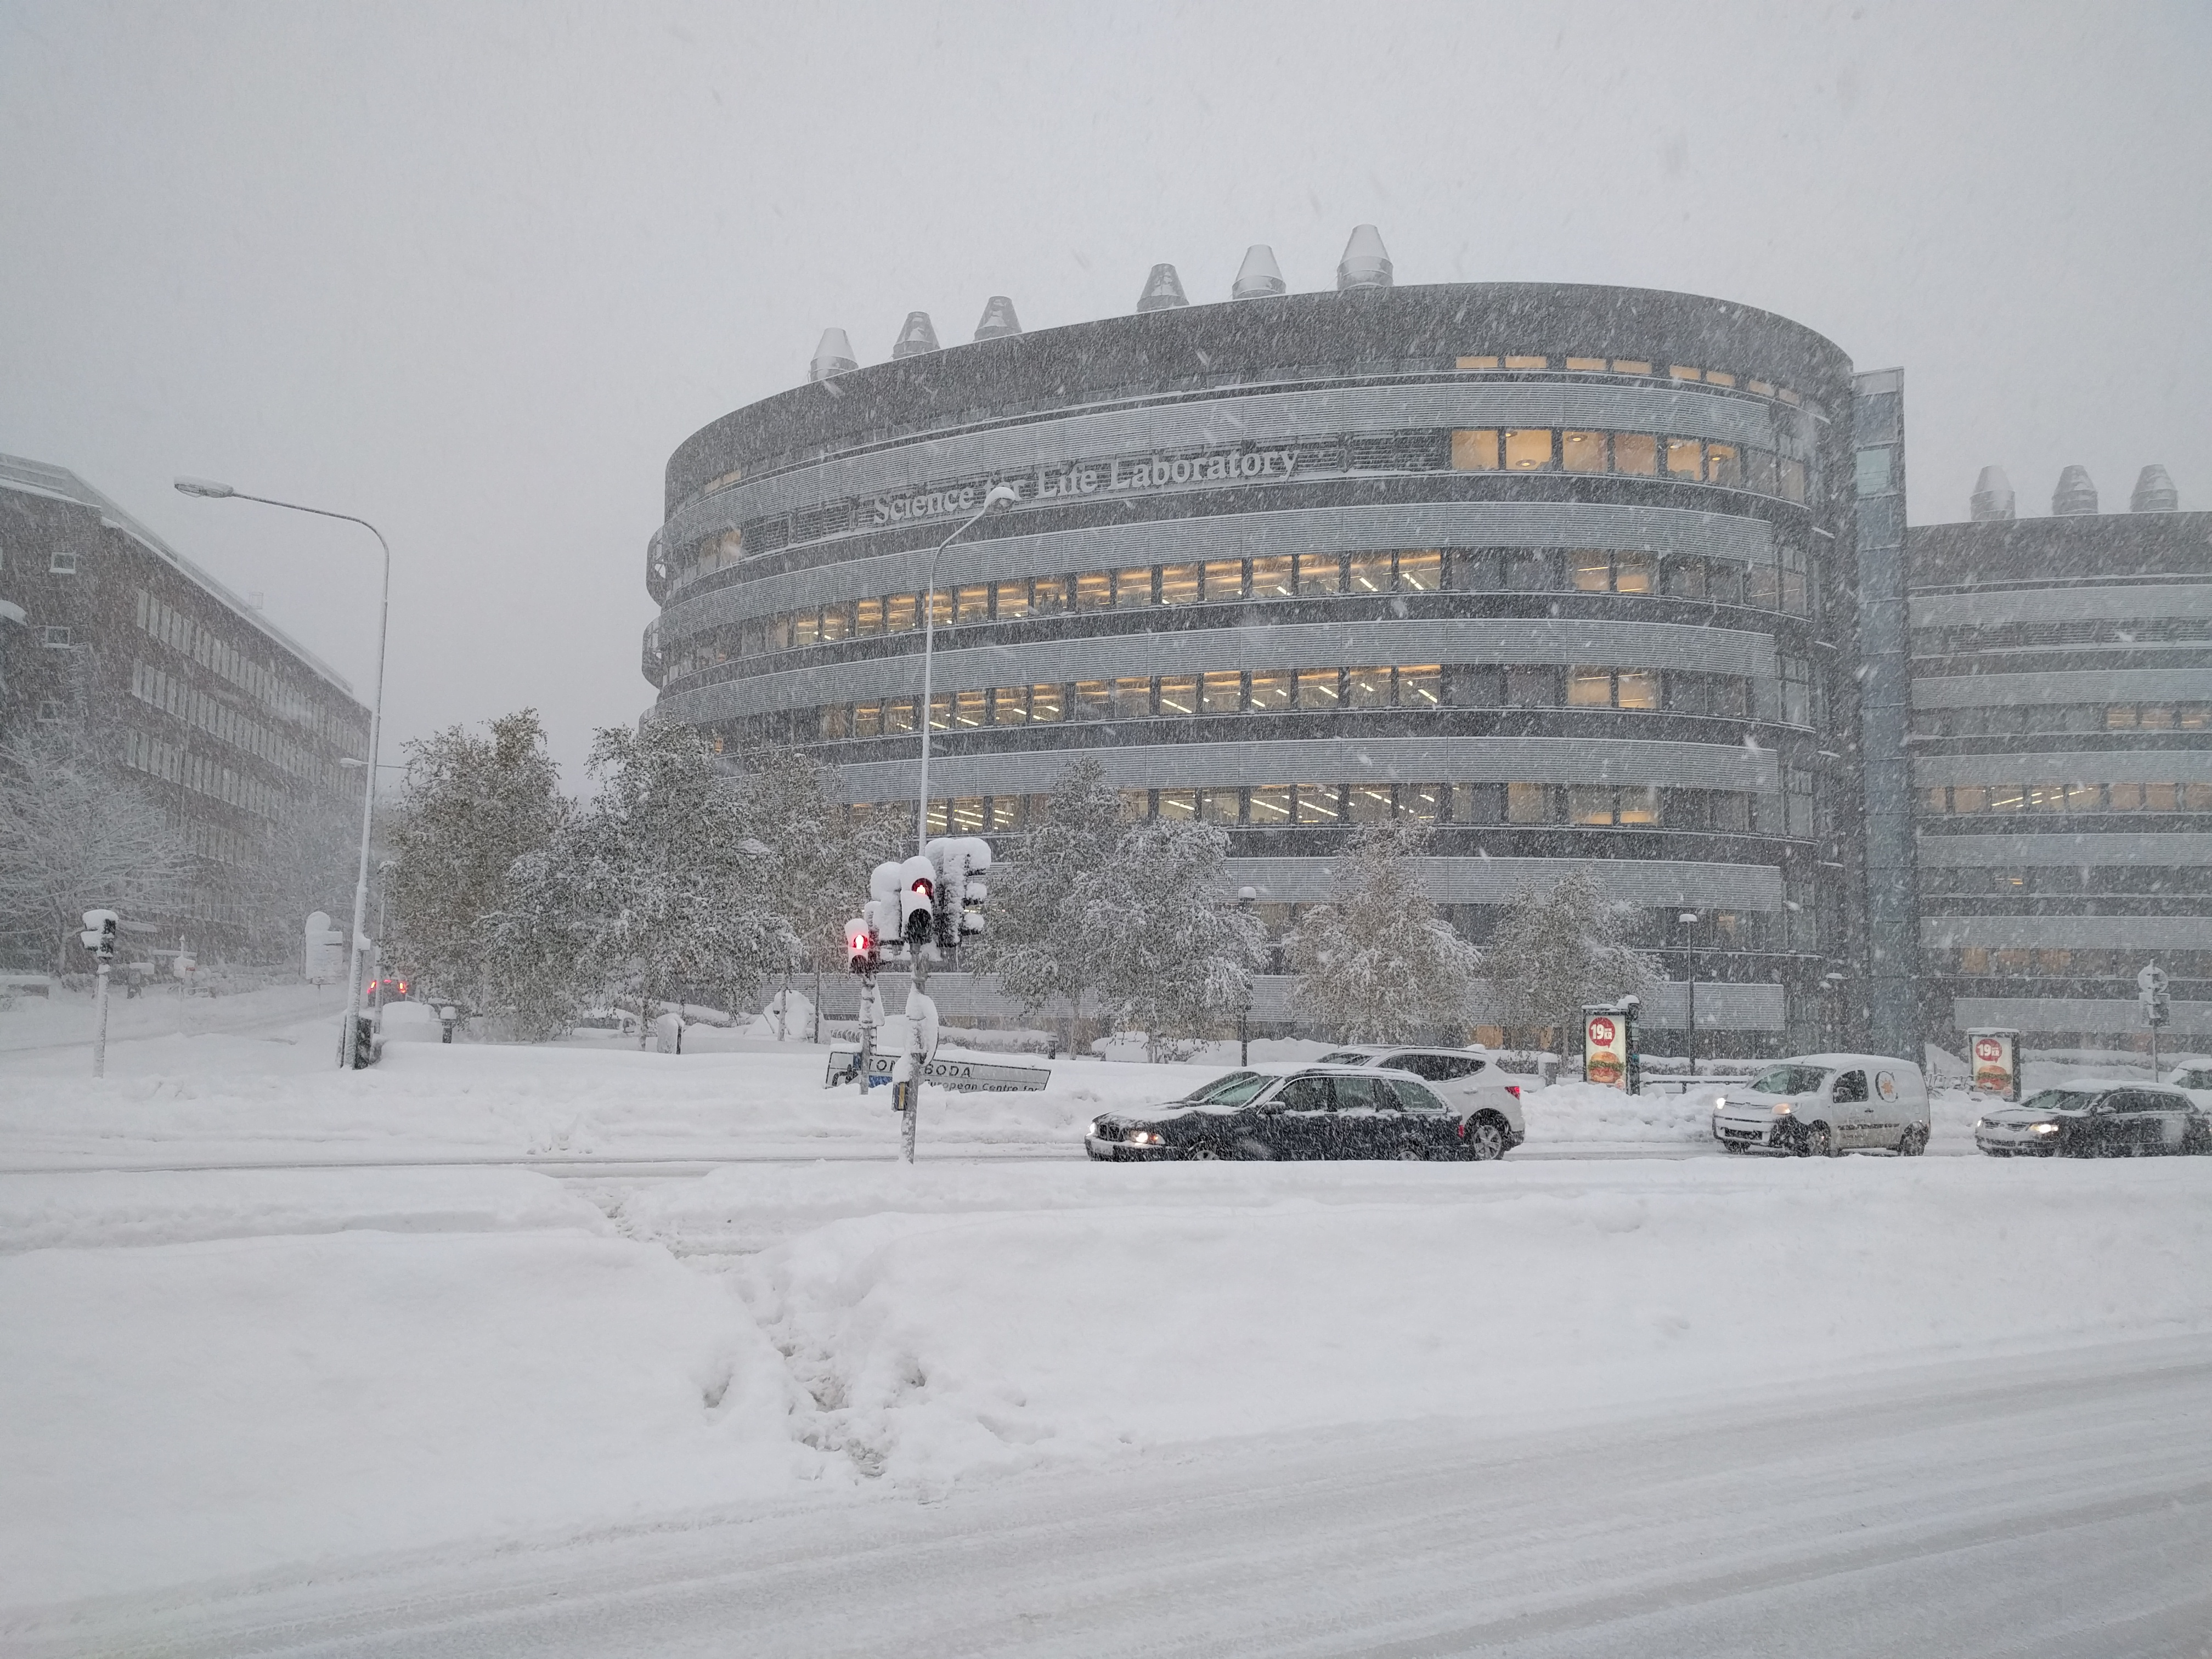
\includegraphics[width=.8\linewidth]{pictures/Snowpocalypse-SciLifeLab.jpg}
	\end{center}
\end{frame}

\end{document}